\chapter{I numeri finiti}
\section{Base-N and Binary}

I numeri hanno diversi modi per essere rappresentati, tra cui quello più comune che è la \textbf{rappresentazione decimale}, dove ogni numero è formato da una lista di caratteri compresi tra $[0,9]$ dove ad ogni cifra è associata una potenza del 10
\\
\esempio{
    \textbf{Esempio}: $147.3 = 1 \cdot 10^2 + 4 \cdot 10^1 + 7 \cdot 10 ^0 + 3 \cdot 10^{-1}$ 
}

In generale, comunque, per convertire un numero da una base \textit{n} a base 10:
\teorema{
    Dato un numero in base \(n\) \( (a_k a_{k-1} \dots a_1 a_0)_n \), la sua conversione in base 10 è data dalla formula:

    \[
    \sum_{i=0}^{k} a_i \cdot n^i
    \]

    dove \(a_i\) sono le cifre in base \(n\) e \(n\) è la base.

}

Per forza di cose i calcolatori operano con i numeri \textit{in base 2}, le cui cifre vengono chiamate\textbf{bit}, esempio $101101$ (base 2).
Per convertire un numero dalla base 10 alle base bisogna dividerlo in potenze di due 
\esempio{
    \[
        37 \, (\text{base } 10) = 32 + 4 + 1 = 1 \cdot 2^5 + 0 \cdot 2^4 + 0 \cdot 2^3 + 1 \cdot 2^2 + 0 \cdot 2^1 + 1 \cdot 2^0 = 100101 \, (\text{base } 2)
    \]
}

In generale occorre dividerlo per due finchè non si riduce ad uno ad esempio: 
\[
(35)_{10} = (100011)_2
\]

\begin{align*}
    35 : 2 &= 17 \quad \text{resto } 1 \\
    17 : 2 &= 8  \quad \text{resto } 1 \\
    8 : 2  &= 4  \quad \text{resto } 0 \\
    4 : 2  &= 2  \quad \text{resto } 0 \\
    2 : 2  &= 1  \quad \text{resto } 0 \\
    1 : 2  &= 0  \quad \text{resto } 1
    \end{align*}
    
    % Creiamo la freccia accanto a tutto l'insieme di divisioni
    \begin{tikzpicture}[overlay, remember picture]
        \draw[->, red, thick] (5.5,1) -- (5.5,-5.5);
    \end{tikzpicture}


\subsection{Addizione e moltiplicazione in binario}
\subsection{Conversione fra basi}
\subsection{Floating point}
Data la finitezza della memoria di un calcolatore, e' impossibile rappresentare esattamente un numero che ha precisione infinita. Per riuscire a rappresentare in modo piu' efficente possibile si usano i \textbf{floating point} numbers:
\dfn{Floating Point}{
  Alloca:
  \begin{itemize}
    \item Un indicatore per il segno ($ s $)
  \item L'esponente ($ e $)
  \item La mantissa ($ f $)
  \end{itemize}
}

Nello standard \textbf{IEEE754} double precision, che occupa 64 bit, un numero e' rappresentato nel seguente modo:
\begin{center}
    no puede soportar este sufrimento
  %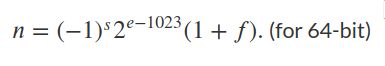
\includegraphics[width=0.5\textwidth]{img/2024-09-16-14-02-10.png}

\end{center}

In generale, ogni numero reale $ n \in \mathbb{R} $ e' definito da:
\begin{center}
    no puede soportar este sufrimento
  %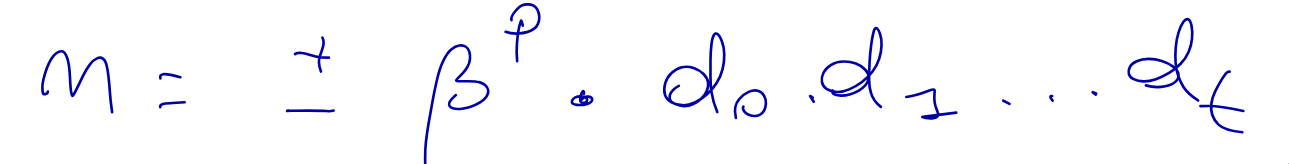
\includegraphics[width=0.5\textwidth]{img/2024-09-16-14-03-42.png}
\end{center}

Quindi l'insieme dei numeri floating point caratterizzati dai valori $ \beta, t, +L, U $ sono:
\begin{center}
    no puede soportar este sufrimento
  %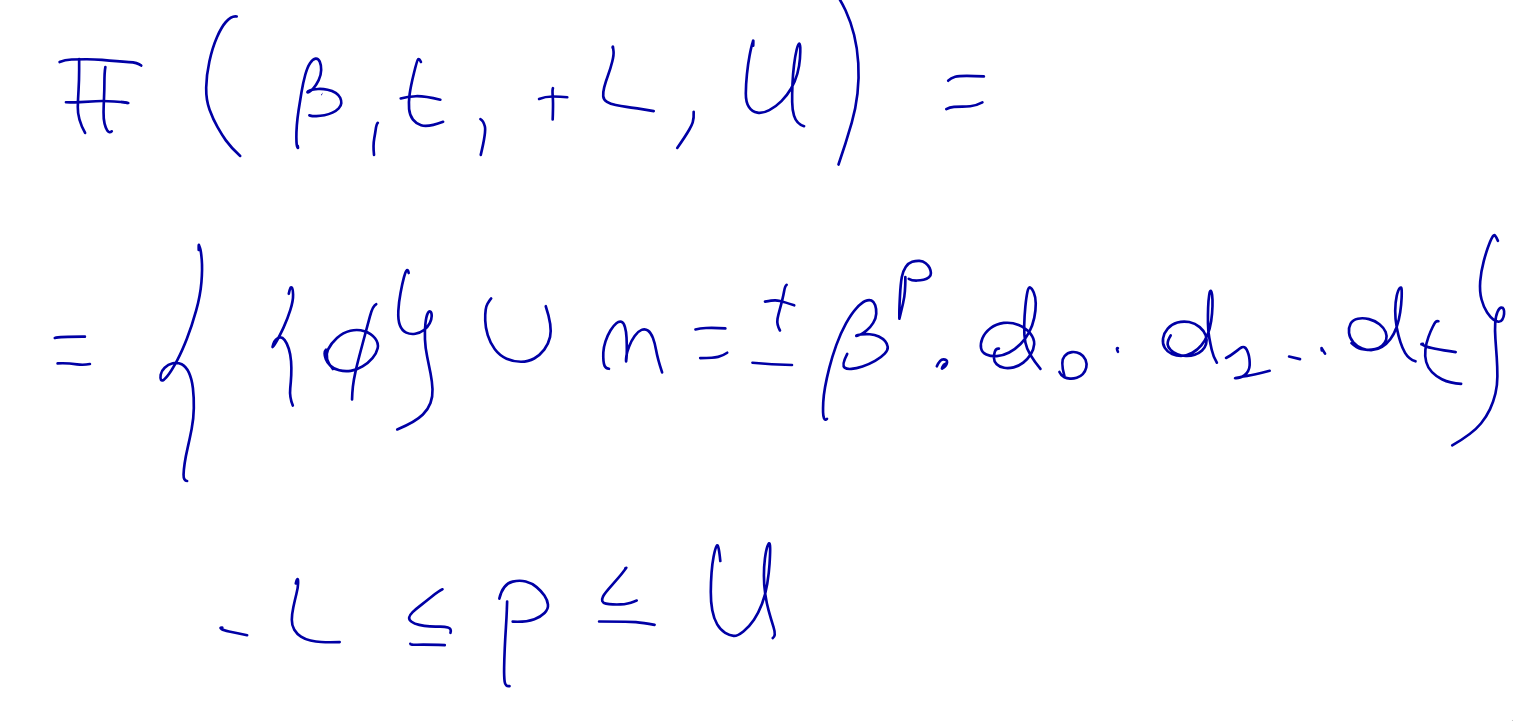
\includegraphics[width=0.5\textwidth]{img/2024-09-16-14-09-02.png}

\end{center}

Se un numero $ x \in \mathbb{R} $ ha un numero di cifre decimali maggiore di $ t $, allora $ x \not\in \mathcal{F} $ e deve essere approssimato (solitamente col troncamento).

\section{Errori di rappresentazione}
Dato che stiamo usando lo stesso numero di bit, il numero di valori rappresentabili rimane uguale, ma la codifica \textit{floating point} fa in modo che il \textbf{gap}, ovvero la differenza, fra due numeri successivi (che esistono sempre dato che lavoriamo con valori discreti) sia relativo al valore assoluto dei numeri rappresentati. Questo e' utile dato che riusciamo ad essere molto precisi con numeri piccoli, riuscendo comunque a rappresentare valori enormi con un errore che in confronto rimane minuscolo. 
\begin{center}
    no puede soportar este sufrimento
  %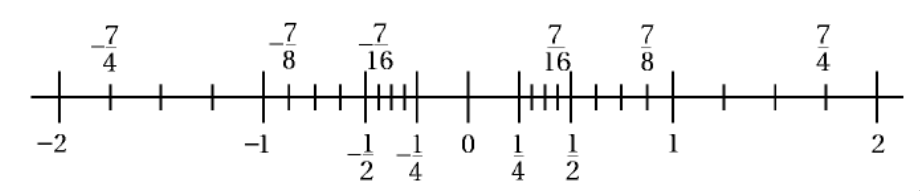
\includegraphics[width=0.5\textwidth]{img/2024-09-22-16-37-40.png}

\end{center}
Abbiamo due modi per indicare l'accuratezza con la quale possiamo rappresentare un valore $ x \in \mathbb{R} $:
\begin{itemize}
\item L'errore \textbf{assoluto}, che e' piu' grande piu' e' grande l'ordine di $ x $
  \[
    |fl(x)-x|<\\beta^{p-t}
  \]
\item E quello \textbf{relativo}, che dipende solo da $ t $
  \[
    \frac{|fl(x)-x|}{|x|} < \frac{1}{2}\beta^{1-t} = \text{\textbf{eps}}
  \]
\end{itemize}
Il valore \textbf{eps} e' detto \textbf{precisione macchina}, ed e' il numero macchina piu' piccolo positivo tale che
\[
  fl(1+\text{eps}) > 1
\]
Quindi, definite due operazioni generiche, una per i reali e l'altra per i floating-point:
\begin{itemize}
\item $ \cdot: \mathbb{R} \times \mathbb{R} \to \mathbb{R} $
\item $ \circ: \mathbb{F} \times \mathbb{F} \to \mathbb{F} $
  \[
    x \circ y = fl(x \cdot y)
  \]
\end{itemize}
Abbiamo che ogni operazione fra floating-point genera un errore (di \textbf{arrotondamento}):
\[
  \left|\frac{(x \circ y) - (x \cdot y)}{x \cdot y}\right| < \text{eps}
\]  
Nel caso di somma di numeri di grandezza molto diversa, le cifre piu' significative del numero piu' piccolo possono essere perse. Per una sola operazione questo non causa un errore troppo grande, ma se l'operazione viene eseguita molte volte l'errore si \textbf{amplifica} e puo' diventare catastrofico.
